\documentclass[aspectratio=169]{beamer}

\setbeamersize{text margin left=5mm, text margin right=5mm}

\defbeamertemplate{headline}{my header}{%
\vskip1pt%
\makebox[0pt][l]{\,\insertshortauthor}%
\hspace*{\fill}\insertshorttitle/\insertshortsubtitle\hspace*{\fill}%
\llap{\insertpagenumber/\insertpresentationendpage\,}
}
\setbeamertemplate{headline}[my header]

\let\olditem\item
\renewcommand{\item}{\setlength{\itemsep}{\fill}\olditem}

\usepackage{caption}
\usepackage{soul}
\usepackage{tkz-euclide}
\usetikzlibrary{calc}
\usepackage[]{algorithm2e}
\usepackage{changepage}
\usepackage{amssymb}
\usepackage{xcolor}
\usepackage{mathtools}
\usepackage{tcolorbox}
\usepackage{tikz}
\usepackage{tikz-3dplot}
\usepackage{tkz-euclide}
\usepackage{circuitikz}
\usepackage{mleftright}
\usetikzlibrary{arrows.meta, decorations.pathreplacing, positioning, shapes.geometric}

%% Fonts
\usefonttheme{professionalfonts}
\usefonttheme{serif}

\DeclareCaptionLabelFormat{blank}{}
\captionsetup[figure]{labelformat=blank}

%% Math definitions
\def\mf{\ensuremath\mathbf}
\def\mb{\ensuremath\mathbb}
\def\mc{\ensuremath\mathcal}
\def\lp{\ensuremath\left(}
\def\rp{\ensuremath\right)}
\def\lv{\ensuremath\left\lvert}
\def\rv{\ensuremath\right\rvert}
\def\lV{\ensuremath\left\lVert}
\def\rV{\ensuremath\right\rVert}
\def\lc{\ensuremath\left\{}
\def\rc{\ensuremath\right\}}
\def\ls{\ensuremath\left[}
\def\rs{\ensuremath\right]}
\def\bmx{\ensuremath\begin{bmatrix*}[r]}
\def\emx{\ensuremath\end{bmatrix*}}
\def\bmxc{\ensuremath\begin{bmatrix*}[c]}
\def\t{\lp t\rp}
\def\k{\ls k\rs}

\newcommand{\demoex}[2]{\onslide<#1->\begin{color}{black!60} #2 \end{color}}
\newcommand{\demoexc}[3]{\onslide<#1->\begin{color}{#2} #3 \end{color}}
\newcommand{\anim}[3]{\onslide<#1->{\begin{color}{#2!60} #3 \end{color}}}
\newcommand{\ct}[1]{\lp #1\rp}
\newcommand{\dt}[1]{\ls #1\rs}
\newcommand{\cols}[2]{\begin{columns}[#1] #2 \end{columns}}
\newcommand{\col}[2]{\begin{column}{#1} #2 \end{column}}

%% Mycolors
\definecolor{myred}{RGB}{192,0,0}
\definecolor{mygray}{RGB}{100,100,100}

%% Custom beamer color
\setbeamercolor{title}{fg=myred}
\setbeamercolor{subtitle}{fg=myred}
\setbeamerfont{title}{series=\bfseries}
% \setbeamercolor{frametitle}{bg=myred, fg=white}
\setbeamercolor{frametitle}{bg=mygray!10!, fg=myred}
\setbeamerfont{frametitle}{series=\bfseries}
\setbeamercolor{item}{fg=mygray}
\setbeamercolor{title in head/foot}{fg=myred}

% Move header to footer
\setbeamertemplate{headline}{}
\setbeamertemplate{footline}{
  \begin{beamercolorbox}[wd=\paperwidth,ht=2.25ex,dp=1ex,center]{footline}
    \inserttitle\hfill\insertauthor\hfill\insertdate\hfill\insertframenumber{}
  \end{beamercolorbox}
}


\title{Applied Linear Algebra in Data Analysis}

% A subtitle is optional and this may be deleted
\subtitle{Matrix Inverses}

\author{Sivakumar Balasubramanian}
% - Give the names in the same order as the appear in the paper.
% - Use the \inst{?} command only if the authors have different
%   affiliation.

\institute[Christian Medical College] % (optional, but mostly needed)
{
  \inst{}%
  Department of Bioengineering\\
  Christian Medical College, Bagayam\\
  Vellore 632002
}
% - Use the \inst command only if there are several affiliations.
% - Keep it simple, no one is interested in your street address.

\date{}
% - Either use conference name or its abbreviation.
% - Not really informative to the audience, more for people (including
%   yourself) who are reading the slides online

\subject{Lecture notes on ALADA}
% This is only inserted into the PDF information catalog. Can be left
% out. 

% If you have a file called "university-logo-filename.xxx", where xxx
% is a graphic format that can be processed by latex or pdflatex,
% resp., then you can add a logo as follows:

% \pgfdeclareimage[height=0.5cm]{university-logo}{university-logo-filename}
% \logo{\pgfuseimage{university-logo}}

% Delete this, if you do not want the table of contents to pop up at
% the beginning of each subsection:
\AtBeginSubsection[]
{
  \begin{frame}<beamer>{Outline}
    \tableofcontents[currentsection,currentsubsection]
  \end{frame}
}

% Let's get started
\begin{document}

\begin{frame}
  \titlepage
\end{frame}

% \begin{frame}[t]{References}
% \begin{itemize}
%   \item S Boyd, Applied Linear Algebra: Chapters 11.
%   \item G Strang, Linear Algebra: Chapters 1.
% \end{itemize}
% \end{frame}


\begin{frame}[t]{Representation of vectors in a basis}
\begin{itemize}
\item Consider the vector space $\mb{R}^n$ with basis $\left\{\mf{v}_1, \mf{v}_2, \ldots \mf{v}_n\right\}$. Any vector in $\mf{b} \in \mb{R}^n$ can be representated as a linear combination of $\mf{v}_i$s,
\[ \mf{b} = \sum_{i=1}^{n} \mf{v}_i\mf{a}_i = \mf{V}\mf{a}; \,\,\, \mf{a} \in \mb{R}^n, \,\,\, \mf{V} = \begin{bmatrix*}\mf{v}_1 & \mf{v}_2 & \ldots & \mf{v}_n\end{bmatrix*} \in \mb{R}^{n \times n} \]

\begin{center}
\begin{minipage}{.3\textwidth}
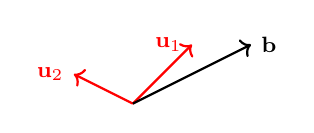
\begin{tikzpicture}[scale=0.75]
  \draw[red,thick,->] (0, 0) -- (1, 1) node[red, above, left]{{\footnotesize $\mf{u}_1$}};
  \draw[red,thick,->] (0, 0) -- (-1, 0.5) node[red, above, left]{{\footnotesize $\mf{u}_2$}};
  \draw[black,thick,->] (0, 0) -- (2, 1) node[black, above, right]{{\footnotesize $\mf{b}$}};
\end{tikzpicture}
\end{minipage}
\begin{minipage}{.3\textwidth}
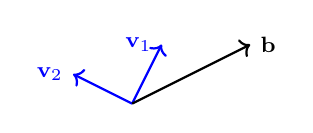
\begin{tikzpicture}[scale=0.75]
  \draw[blue,thick,->] (0, 0) -- (0.5, 1) node[blue, above, left]{{\footnotesize $\mf{v}_1$}};
  \draw[blue,thick,->] (0, 0) -- (-1, 0.5) node[blue, above, left]{{\footnotesize $\mf{v}_2$}};
  \draw[black,thick,->] (0, 0) -- (2, 1) node[black, above, right]{{\footnotesize $\mf{b}$}};
\end{tikzpicture}
\end{minipage}
\begin{minipage}{.3\textwidth}
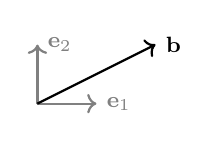
\begin{tikzpicture}[scale=0.75]
  \draw[gray,thick,->] (0, 0) -- (1, 0) node[gray, above, right]{{\footnotesize $\mf{e}_1$}};
  \draw[gray,thick,->] (0, 0) -- (0, 1) node[gray, above, right]{{\footnotesize $\mf{e}_2$}};
  \draw[black,thick,->] (0, 0) -- (2, 1) node[black, above, right]{{\footnotesize $\mf{b}$}};
\end{tikzpicture}
\end{minipage}
\end{center}
$\left\{\mf{v}_1, \mf{v}_2\right\}$, $\left\{\mf{u}_1, \mf{u}_2\right\}$ and $\left\{\mf{e}_1, \mf{e}_2\right\}$ are valid basis for $\mb{R}^2$, and the presentation for $\mf{b}$ in each one of them is different.
\end{itemize}
\end{frame}


\begin{frame}[t]{Matrix Inverse}
\begin{itemize}
    \item Consider the equation $\mf{Ax} = \mf{y}$, where $\mf{A} \in \mb{R}^{n \times n}$ and $\mf{x}, \mf{y} \in \mb{R}^n$. 

    \item Let us assume $\mf{A}$ is non-singular $\implies$ columns of $\mf{A}$ represent a basis for $\mb{R}^n$.

    \item What does $\mf{x}$ represent? It is the representation of $\mf{y}$ in the basis consisitng of the columns of $\mf{A}$.
    \[ \mf{y} = \mf{Ax} = \begin{bmatrix*}\mf{a}_1 & \mf{a}_2 & \ldots & \mf{a}_n\end{bmatrix*}\begin{bmatrix*}x_1 \\ x_2 \\ \vdots \\ x_n\end{bmatrix*} = \sum_{i=1}^{n}\mf{a}_i x_i\]
    \[ \implies \,\, \mf{x} = \mf{A}^{-1}\mf{y} = \begin{bmatrix*}\tilde{\mf{b}}_1^\top \\ \tilde{\mf{b}}_2^\top \\ \ldots \\ \tilde{\mf{b}}_n^\top\end{bmatrix*}\mf{y} = \begin{bmatrix*}\tilde{\mf{b}}_1^\top\mf{y} \\ \tilde{\mf{b}}_2^\top\mf{y} \\ \ldots \\ \tilde{\mf{b}}_n^\top\mf{y}\end{bmatrix*} \]
\end{itemize}
\end{frame}

\begin{frame}[t]{Matrix Inverse}
\begin{itemize}
    \item $\mf{A}^{-1}$ is a matrix that allows change of basis to the columns of $\mf{A}$ from the standard basis!
\end{itemize}
\vspace{1cm}

% \begin{color}{blue}
%     $\bullet$ $W = \lc \begin{bmatrix*}[r]1\\1\end{bmatrix*}, \begin{bmatrix*}[r]-1\\\frac{1}{2}\end{bmatrix*} \rc$. Find $\mf{b}_W$ by calculating the inverse of the matrix $\mf{W} = \begin{bmatrix*}[r]1 & -1\\1 & \frac{1}{2}\end{bmatrix*}$.\\ \vspace{0.2cm}

%     $\bullet$ What about $V = \lc \begin{bmatrix*}[r]\sfrac{1}{\sqrt{5}}\\\sfrac{2}{\sqrt{5}}\end{bmatrix*}, \begin{bmatrix*}[r]-\sfrac{2}{\sqrt{5}}\\\sfrac{1}{\sqrt{5}}\end{bmatrix*} \rc$. What is $\mf{b}_V$?
% \end{color}
\end{frame}


% \begin{frame}[t]{Matrix Inverse}
% \vspace{-0.25cm}
% \begin{columns}
% \begin{column}{0.5\textwidth}
% \vspace{-0.2cm}
% \begin{center}
% \begin{tikzpicture}[scale=1.1]
%     % xy grid
%     \draw[step=0.25, gray!20!, thin, xshift=0cm, yshift=0cm] (-2.5,-0.25) grid (2.5,2);
%     \draw[gray!25!,thin] (-2.5,0) -- (2.5,0);
%     \draw[gray!25!,thin] (0,-1) -- (0,2);
%     \draw[black!80!, thin, ->] (0,0) -- (1,0) node[black!80!, right] {{\tiny $\mf{e}_1$}};
%     \draw[black!80!, thin, ->] (0,0) -- (0,1) node[black!80!, above] {{\tiny $\mf{e}_2$}};
%     \draw[blue, thin, ->] (0,0) -- (2, 1) node[xshift=-0.2cm, yshift=-0.5cm] {{\tiny $\mf{v}_1 = \left[2,\,1\right]^\top$}};
%     \draw[blue, thin, ->] (0,0) -- (-1, 1/2) node[xshift=-0.4cm, yshift=0.3cm] {{\tiny $\mf{v}_2 = \left[-1,\,\frac{1}{2}\right]^\top$}};
%     \draw[red, thin, ->] (0,0) -- (1/4, 1/2) node[xshift=0.5cm,yshift=0.5cm] {\rotatebox{30}{\tiny $\tilde{\mf{u}}_1^\top = \left[\frac{1}{4},\,\frac{1}{2}\right]$}};
%     \draw[red, thin, ->] (0,0) -- (-1/2, 1) node[xshift=-0.75cm, yshift=0.3cm] {{\tiny $\tilde{\mf{u}}_2^\top = \left[-\frac{1}{2},\,1\right]$}};
%     \node[above] at (0,1.6) {{\small Columns of $\mf{A}$ and rows of $\mf{A}^{-1}$}};
% \end{tikzpicture}

% \vspace{-0.5cm}
% \begin{tikzpicture}[scale=1.1]
%     % xy grid
%     \draw[step=0.25, gray!20!, thin, xshift=0cm, yshift=0cm] (-2.5,-1) grid (2.5,2);
%     \draw[gray!25!,thin] (-2.5,0) -- (2.5,0);
%     \draw[gray!25!,thin] (0,-1) -- (0,2);
%     \draw[black!80!, thin, ->] (0,0) -- (1,0) node[black!80!, right] {{\tiny $\mf{e}_1$}};
%     \draw[black!80!, thin, ->] (0,0) -- (0,1) node[black!80!, above] {{\tiny $\mf{e}_2$}};
%     \draw[blue, thin, ->] (0,0) -- (2, -1) node[xshift=-0.4cm, yshift=0.6cm] {{\tiny $\tilde{\mf{v}}_1^\top = \left[2,\,1\right]$}};
%     \draw[blue, thin, ->] (0,0) -- (1, 1/2) node[xshift=0.3cm, yshift=0.3cm] {{\tiny $\tilde{\mf{v}}_2 = \left[-2,\,\frac{1}{2}\right]^\top$}};
%     \draw[red, thin, ->] (0,0) -- (1/2, -1) node[xshift=-1.2cm,yshift=0.25cm] {{\tiny $\mf{u}_1 = \left[\frac{1}{2},\,-1\right]^\top$}};
%     \draw[red, thin, ->] (0,0) -- (1, 2) node[xshift=-0.9cm, yshift=-0.3cm] {{\tiny $\mf{u}_2 = \left[1,\,2\right]^\top$}};
%     \node[above] at (0,2.1) {{\small Rows of $\mf{A}$ and columns of $\mf{A}^{-1}$}};
% \end{tikzpicture}
% \end{center}
% \end{column}

% \begin{column}{0.5\textwidth}
% \[ \mf{V} = \begin{bmatrix*}\mf{v}_1 & \mf{v}_2\end{bmatrix*} = \begin{bmatrix*}[r]2 & -1\\1 & \frac{1}{2}\end{bmatrix*}\]

% \[ \mf{V}^{-1} = \begin{bmatrix*}\tilde{\mf{u}}_1^\top \\ \tilde{\mf{u}}_2^\top\end{bmatrix*} = \frac{1}{2}\begin{bmatrix*}[r]\frac{1}{2} & 1\\-1 & 2\end{bmatrix*}\]

% \[ \mf{v}_1^\top\tilde{\mf{u}}_1 = \mf{v}_2^\top\tilde{\mf{u}}_2 = \tilde{\mf{v}}_1^\top\mf{u}_1 = \tilde{\mf{v}}_2^\top\mf{u}_2 = 1 \]

% \[ \mf{v}_1^\top\tilde{\mf{u}}_2 = \mf{v}_2^\top\tilde{\mf{u}}_1 = \tilde{\mf{v}}_1^\top\mf{u}_2 = \tilde{\mf{v}}_2^\top\mf{u}_1 = 0 \]

% \vspace{0.25cm}
% \demoex{2}{
% Verify these for $\mf{W} = \begin{bmatrix*}[r]1 & -1\\1 & \frac{1}{2}\end{bmatrix*}$ and $\mf{V} = \begin{bmatrix*}[r]\sfrac{1}{\sqrt{5}} & -\sfrac{2}{\sqrt{5}}\\\sfrac{2}{\sqrt{5}} & \sfrac{1}{\sqrt{5}}\end{bmatrix*}$.
% }

% \end{column}
% \end{columns}
% \end{frame}


\begin{frame}[t]{Left Inverse}
\begin{itemize}
    \item Consider a rectangular matrix $\mf{A} \in \mb{R}^{m \times n}$. There exists no inverse $\mf{A}^{-1}$ for this matrix.

    \item But, there exist two matrices $\mf{B}, \mf{C} \in \mb{R}^{n \times m}$, such that,
    \[ \mf{CA} = \mf{I}_n \,\,\,\,\, \text{ or } \,\,\,\,\, \mf{AB} = \mf{I}_m \]

    \item Both cannot be true for a rectangular matrix, only one can be true when the matrix is full rank.

    \item A rectangular matrix can only have either a left or a right inverse.

\end{itemize}
\end{frame}


\begin{frame}[t]{Right Inverse}
% \vspace{-0.25cm}
\begin{itemize}
    \item For $\mf{A} \in \mb{R}^{m \times n}$, $n > m$ with full rank, $\mf{AB} = \mf{I}_m \longrightarrow \mf{B} \text{ is the right inverse.}$

    \item Right inverse of $\mf{A}$ exists only if the rows of $\mf{A}$ are independent, i.e. $rank\left(\mf{A}\right) = m$ $\longrightarrow \mf{A}^\top\mf{x} = \mf{0} \implies \mf{x} = \mf{0}$

    \item $\mf{Ax} = \mf{b}$ can be solved for any $\mf{b}$. $\mf{x} = \mf{Bb} \implies \mf{A}\left(\mf{Bb}\right) = \mf{b}$. 

    \item There are an infitnite number of $\mf{B}$s $\implies$ an infinite number of solutions $\mf{x}$.
\end{itemize}
\end{frame}


\begin{frame}[t]{Pseudo Inverse}
\begin{itemize}
    \item Consider a tall matrix $\mf{A} \in \mb{R}^{m \times n}$ with independent columns. It turns out the Gram matrix $\mf{A}^\top\mf{A} \in \mb{R}^{n \times n}$ is invertible. If that is the case then,
    \[ \left(\mf{A}^\top\mf{A}\right)^{-1}\mf{A}^\top\mf{A} = \mf{I}_n; \,\,\,\,\, \left(\mf{A}^\top\mf{A}\right)^{-1}\mf{A}^\top \text{ is a left inverse.} \]
    \item $\mf{A}^{\dagger} = \left(\mf{A}^\top\mf{A}\right)^{-1}\mf{A}^\top$ is called the \textit{pseudo inverse} or the \textit{Moore-Penrose inverse}.

    \item For the case of a fat, wide matrix, we have $\mf{A}^{\dagger} = \mf{A}^\top\left(\mf{AA}^\top\right)^{-1}$.

    \item When $\mf{A}$ is square and invertible, $\mf{A}^{\dagger} = \mf{A}^{-1}$.
\end{itemize}
\end{frame}


% \begin{frame}[t]{Pseudo Inverse}
% \begin{color}{blue}
%     $\bullet$ Solve $\mf{Ax} = \mf{b}$ using the $\mf{A}^\dagger$. $\mf{A} = \begin{bmatrix*}[r]1\\2\end{bmatrix*}$, and $\mf{b} = \begin{bmatrix*}2\\4\end{bmatrix*}$. Find $\mf{x}$.\\
%     \vspace{2cm}

%     $\bullet$ Compare $\mf{A}^\dagger$ with that of the general left inverse $\mf{C}$. Calculate $\lV \mf{C} \rV^2$ and find out the $\min \lV\mf{C}\rV^2$. What is $\lV\mf{A}^\dagger\rV^2$?
% \end{color}
% \end{frame}



% \begin{frame}[t]{Pseudo Inverse}
% \begin{color}{blue}
%     $\bullet$ Solve $\mf{Ax} = \mf{b}$ using the $\mf{A}^\dagger$. $\mf{A} = \begin{bmatrix*}[r]1 & 1\end{bmatrix*}$, and $\mf{b} = \begin{bmatrix*}3\end{bmatrix*}$. Find $\mf{x}$.\\
%     \vspace{2cm}

%     $\bullet$ Write down all the possible solution $\mf{x}$. What is the $\mf{x}$ with the smallest length? What is $\mf{A}^\dagger \mf{b}$?
% \end{color}
% \end{frame}


\begin{frame}[t]{Matrix Inverse and Pseudo Inverse through $\mf{QR}$ factorization}
\begin{itemize}
    \item Consider an invertible, square matrix $\mf{A} \in \mb{R}^{n \times n}$. 
    \[ \mf{A} = \mf{QR} \implies \mf{A}^{-1} = \left(\mf{QR}\right)^{-1} = \mf{R}^{-1}\mf{Q}^{-1} = \mf{R}^{-1}\mf{Q}^\top \] 
    where, $\mf{R}, \mf{Q} \in \mb{R}^{n \times n}$. $\mf{R}$ is upper triangular, and $\mf{Q}$ is an orthogonal matrix.
    
    \item In the case of a left invertible rectangular matrix $\mf{A} \in \mb{R}^{m \times n}$, we can factorize $\mf{A} = \mf{QR}$, with $\mf{Q} \in \mb{R}^{m \times n}$ and $\mf{R} \in \mb{R}^{m \times m}$.
    \[ \mf{A}^{\dagger} = \left(\mf{A}^\top\mf{A}\right)^{-1}\mf{A}^\top = \left(\mf{R}^\top\mf{Q}^\top\mf{QR}\right)^{-1}\mf{R}^\top\mf{Q}^\top = \left(\mf{R}^\top\mf{R}\right)^{-1}\mf{R}^\top\mf{Q}^\top = \mf{R}^{-1}\mf{Q}^\top \]
\end{itemize}
\end{frame}


\begin{frame}[t]{Matrix Inverse and Pseudo Inverse through $\mf{QR}$ factorization}
\begin{itemize}
    \item For a right invertible wide, fat matrix, we can find out the pseudo-inverse of $\mf{A}^\top$, and then take the transpose of the pseudo-inverse.
    \[ \mf{AA}^{\dagger} = \mf{I} \implies \left(\mf{A}^{\dagger}\right)^\top\mf{A}^\top = \left(\mf{A}^\top\right)^{\dagger}\mf{A}^\top = \mf{I} \]
    \[ \mf{A}^\top = \mf{QR} \implies \left(\mf{A}^\top\right)^{\dagger} = \mf{R}^{-1}\mf{Q}^\top = \left(\mf{A}^{\dagger}\right)^\top \implies  \mf{A}^{\dagger} = \mf{QR}^{-T} \]
\end{itemize}
\end{frame}


\begin{frame}[t]{What about when $\mf{A}$ is not full rank?}
\begin{itemize}
    \item There is no left or right inverse for $\mf{A} \in \mb{R}^{m \times n}$, when $rank(\mf{A}) = r < \min(m, n)$.
    \[ \nexists \,\, \mf{B} \in \mb{R}^{n \times m}, s.t. \,\, \mf{B}\mf{A} = \mf{I}_m \,\, \text{or} \,\, \mf{AB} = \mf{I}_n \]
    
    \item \textbf{$\mf{A}$ is tall}: First $r$ columns of $\mf{A}$ are linear independent, then  $\exists \,\, \mf{B} \in \mb{R}^{n \times m}, s.t.$
    \[\mf{BA} = \bmx \mf{I}_r & \mf{0} \\ \mf{0} & \mf{0} \emx \]
    
    \item \textbf{$\mf{A}$ is fat}: First $r$ rows of $\mf{A}$ are linear independent, then  $\exists \,\, \mf{B} \in \mb{R}^{n \times m}, s.t.$
    \[\mf{AB} = \bmx \mf{I}_r & \mf{0} \\ \mf{0} & \mf{0} \emx \]
    
\end{itemize}
\end{frame}


\begin{frame}[t]{What about when $\mf{A}$ is not full rank?}
\begin{itemize}
    \item What if we have a linear system of equations with a non-full rank matrix $\mf{A} \in \mb{R}^{m \times n}$?
    \[ \mf{Ax} = \mf{b} \]
    
    \item $\mf{b} \in \mathcal{C}\lp \mf{A} \rp \,\, \implies $ There are infinitely many solutions to the above equation.

    \item $\mf{b} \notin \mathcal{C}\lp \mf{A} \rp \,\, \implies $ There is no solution to the above equation. But there are infinitely many solutions $\hat{\mf{x}}$ that minimize $\Vert \mf{b} - \mf{A}\hat{\mf{x}} \Vert_2$.
    
    \item One approach to solve the case wherre $\mf{b} \notin \mc{C}\lp \mf{A} \rp$ is to formualte the problem as a regularized least squares problem,
    \[ \hat{\mf{x}} = \arg \min \Vert \mf{Ax} - \mf{b}\Vert_2^2 + \lambda \Vert \mf{x} \Vert_2^2 \]
\end{itemize}
\end{frame}

\end{document}